\chapter{Transition entre Colmap et SolAR}

Introduction (Objectif du helper)

\section{Données en entrée et sortie}

Présentation fichiers entrées sortie de Colmap (Images d'entrée, database.db et fichiers de sortie avec infos globales de chaque fichier)

Présentation API SolAR et classes d'entrée et de sortie (datastructure map, point cloud, keyframe collection et Image)

\section{Transition entre Colmap et SolAR}

Présentation des différentes fonctions du helper (entrées/sorties et fonctionnalitées)

\section{Résultats}

Résultats de colmap sur SolAR (Plus de résultats annexe \ref{fig:test_dino} et \ref{fig:test_museum})

\begin{figure}[ht]
    \centering
    \begin{subfigure}{0.45\textwidth}
        \includegraphics[width=\linewidth]{datas/helper/test_keyframe1.png}
    \end{subfigure}
    \begin{subfigure}{0.45\textwidth}
        \includegraphics[width=\linewidth]{datas/helper/test_keyframe2.png}
    \end{subfigure}

    \caption{Résultats des tests de keyframes avec deux points de vue}
    \label{fig:keyframe_canap}
\end{figure}

\addimage{helper/test_descriptors}{Résultats des tests de descriptors}

\begin{figure}[ht]
    \centering
    \begin{subfigure}{0.45\textwidth}
        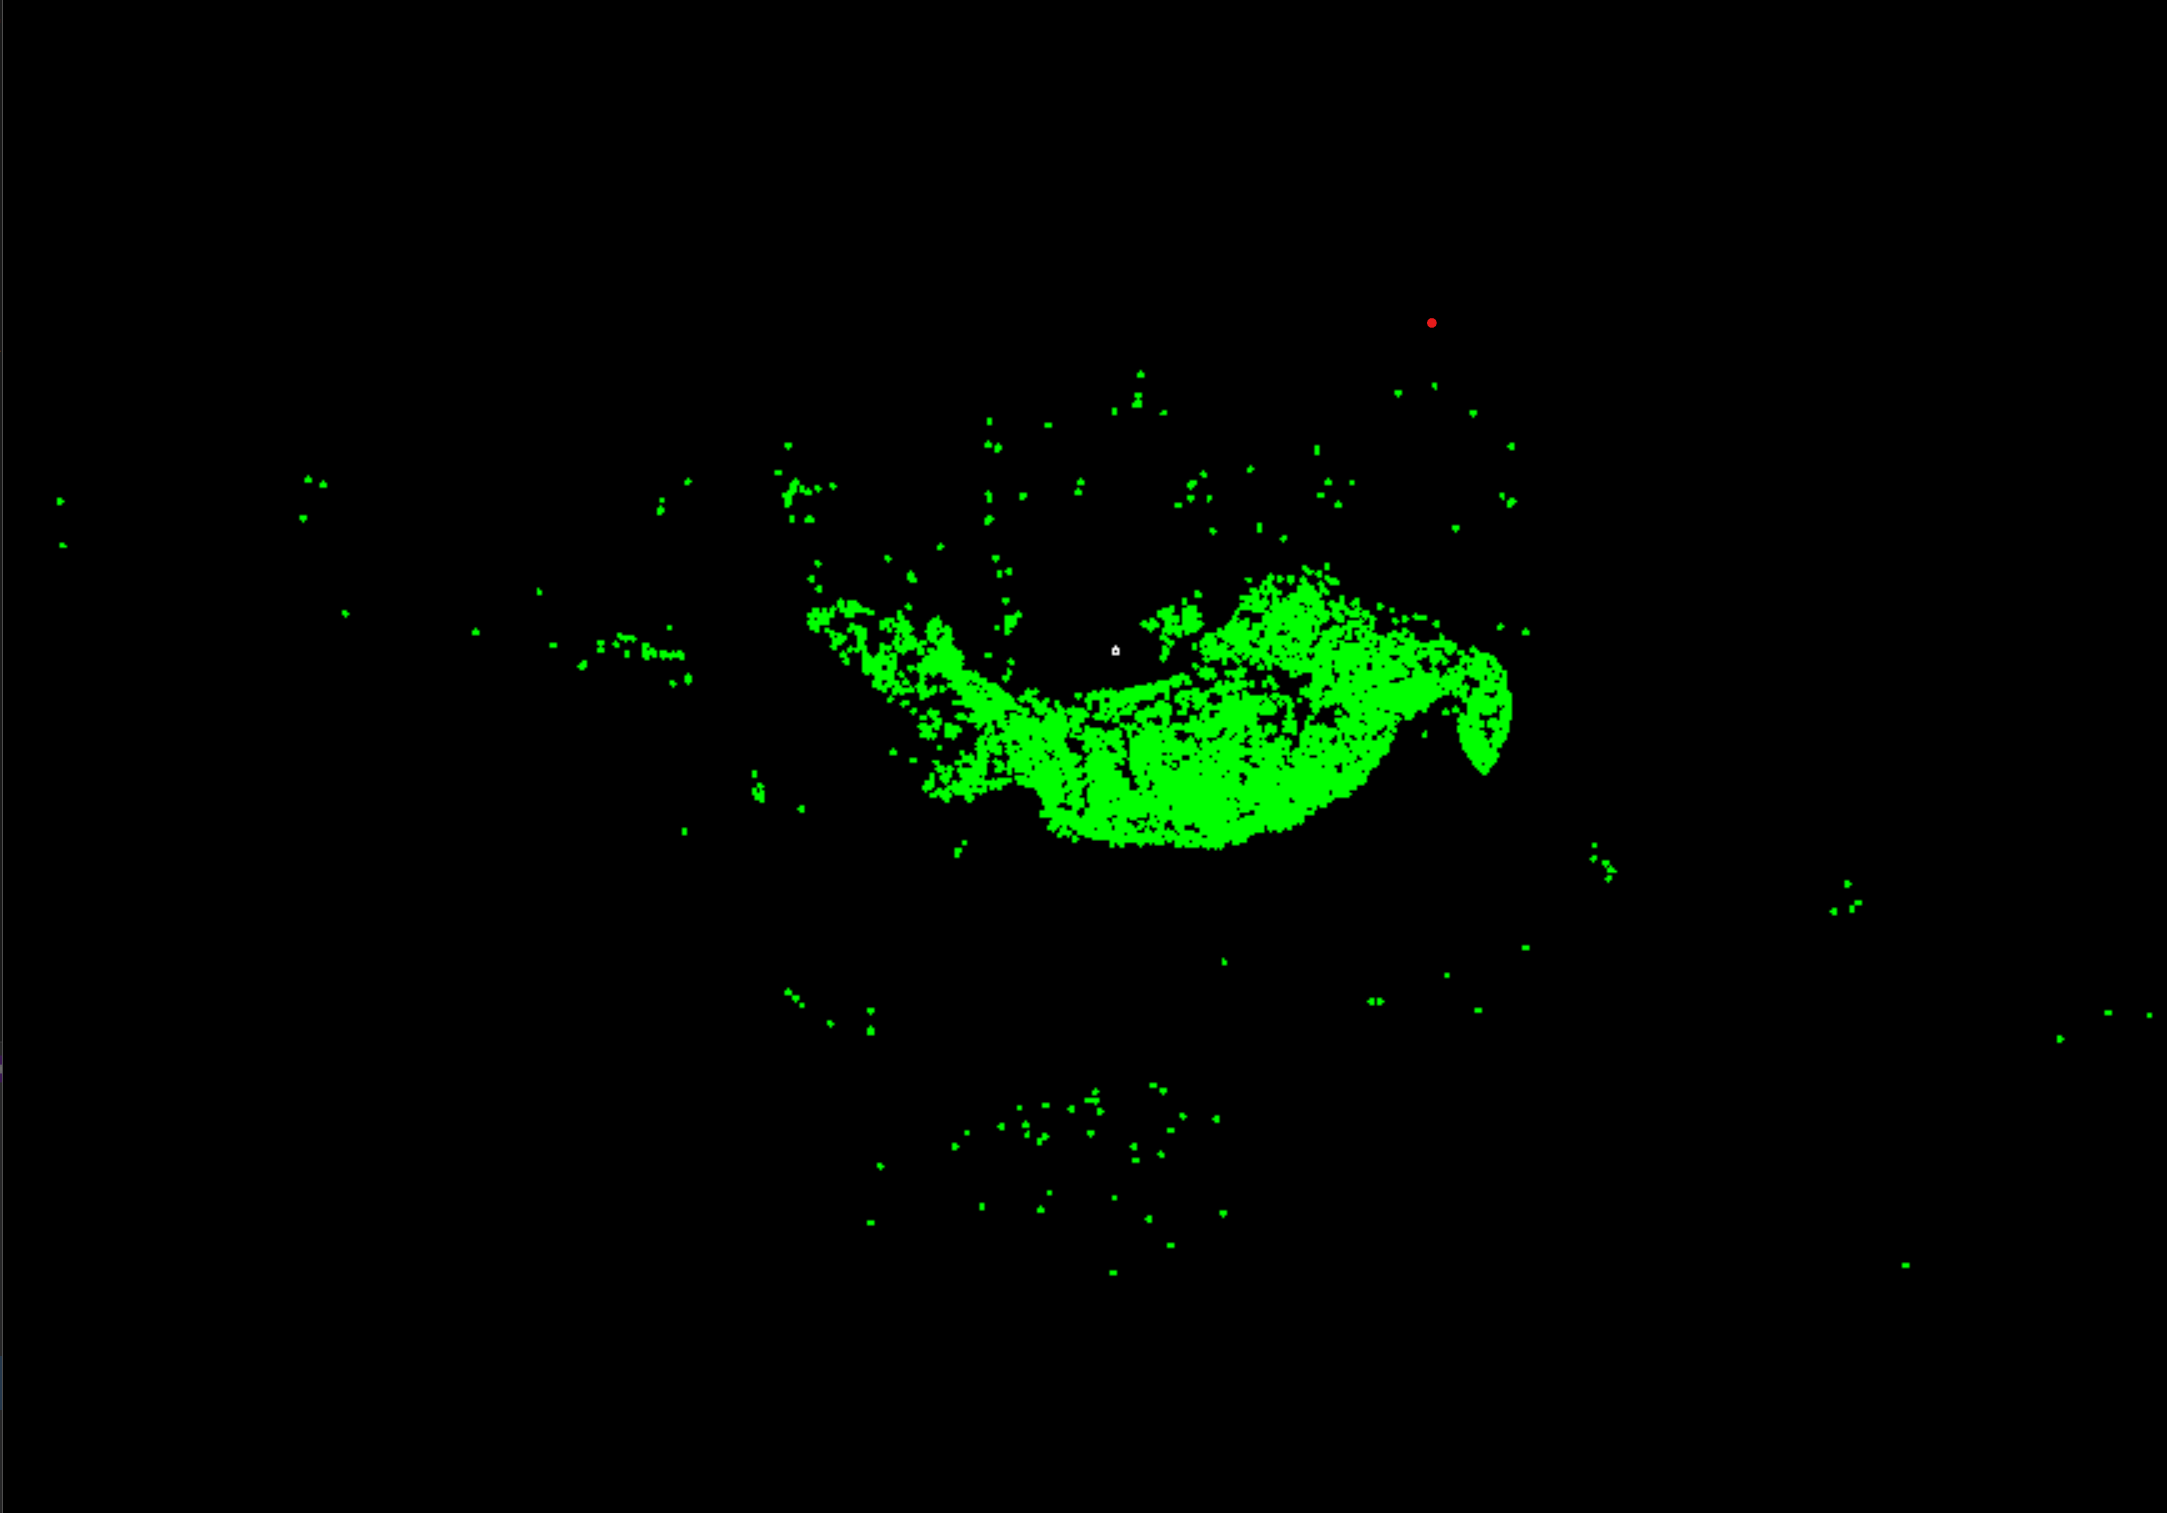
\includegraphics[width=\linewidth]{datas/helper/test_pointcloud.png}
    \end{subfigure}
    \begin{subfigure}{0.45\textwidth}
        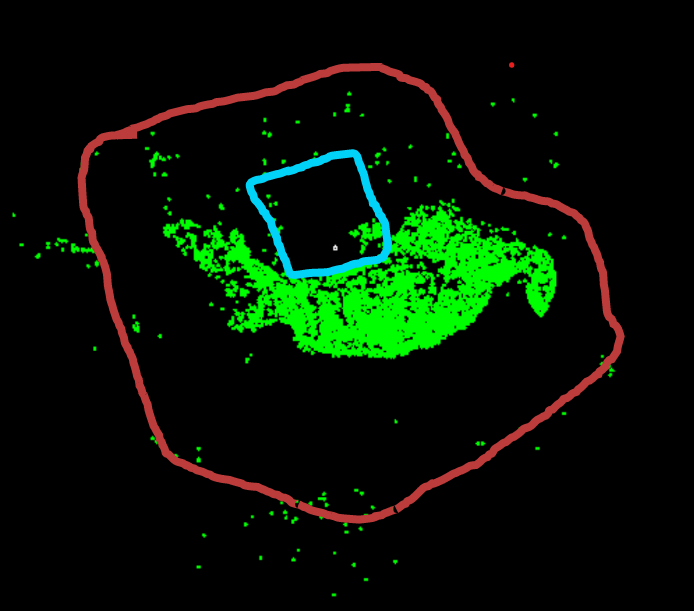
\includegraphics[width=\linewidth]{datas/helper/test_pointcloud_schema.png}
    \end{subfigure}

    \caption{Résultats des tests d'affichage du point cloud (schéma à droite pour identifier la forme du canapé)}
    \label{fig:pointcloud_canap}
\end{figure}